\section{Laboratory work implementation} 

\subsection{Task 1 - Scenario of testing}

I've chosen to test the on online application for calculating integrals which you can find at the link \href{https://www.integral-calculator.com/}{IntCalc}.

The scenario for testing the 3 functionalities is as follows : 

\begin{itemize}
	\item Verify that the input fields are available to insert data and the submit button works as expected;
	\item Check if the output gives the solution for an example;
	\item See if the \textbf{Options} menu permits us to change the parameters;
\end{itemize}

\subsection{Task 2 - Organizational criteria of EC and DT}

The organizational criteria will be the type of input expression and options we introduce.

This way I've obtained the following partitions : 

\begin{itemize}
	\item Valid mathematical expressions and options;
	\item Non-valid expression/Non-valid characters but valid options;
	\item Non-valid expression/options;
\end{itemize}

The decision table :

\begin{table}[h]
	\begin{tabular}{|l|l|l|l|l|}
		\hline
		\multicolumn{1}{|c|}{\textbf{Fields\textbackslash{}Cases}} & \textbf{Case 1} & \textbf{Case 2} & \textbf{Case 3} & \textbf{Case 4} \\ \hline
		\textbf{Expression}      & Valid & Valid  & Non-valid & Non-valid \\ \hline
		\textbf{Options}         & Ok    & Not Ok & Ok        & Not Ok    \\ \hline
		\textbf{Output(Res/Err)} & Res   & Err    & Err       & Err       \\ \hline
	\end{tabular}
\end{table}

\subsection{Task 3 - Conclusive tests}

Test cases and their description : 

\begin{itemize}
	\item Case 1 - A valid mathematical expression and options; \\
		  Example : $cos(x)$; \\
		  Expected : $sin(x) + C$; \\
		  
	\item Case 2 - A valid expression but non-valid options; \\
		  Example : Upper bound = A russian letter; \\
		  Expected : Invalid character; \\
	
	\item Case 3 - A non-valid mathematical expression, but valid options; \\
	   	  Example : $cos(x)/0$; \\
	      Expected : Error; \\
	
	\item Case 4 - A non-valid expression and non-valid options; \\
		  Example : Russian chars at the options and input expression; \\
		  Expected : Error; \\
\end{itemize}

Boundary testing : 

I've introduced the max and min values for Upper and Lower bounds: 

\begin{center}
	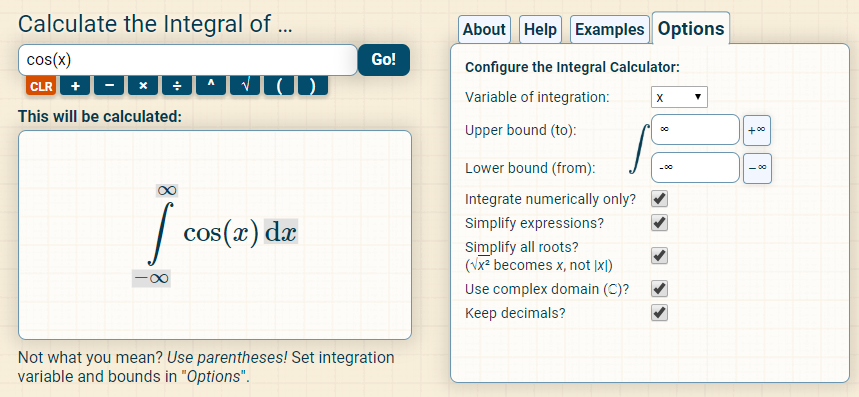
\includegraphics[scale=0.7]{images/Capture2}
\end{center}

Results for the test cases : 


\begin{center}
	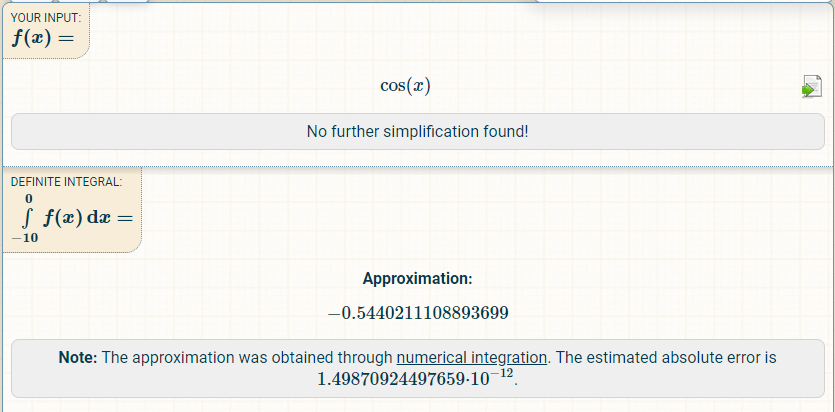
\includegraphics[scale=0.7]{images/Case1}
	\captionof{figure}{Test Case 1}
	\vspace{1cm}
\end{center}


\begin{center}
	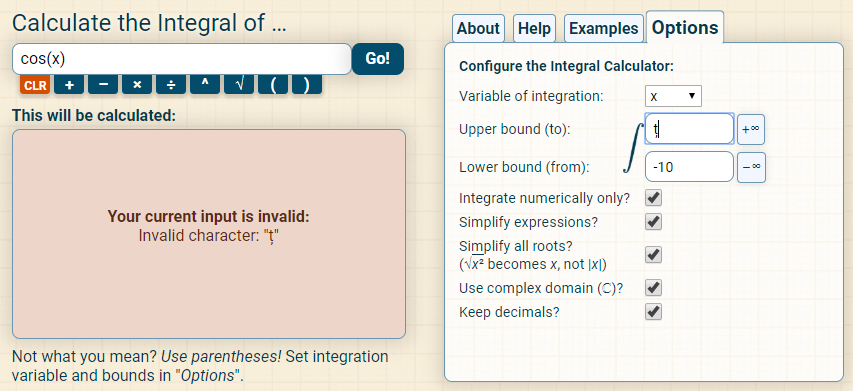
\includegraphics[scale=0.7]{images/Case2}
	\captionof{figure}{Test Case 2}
	\vspace{1cm}
\end{center}


\begin{center}
	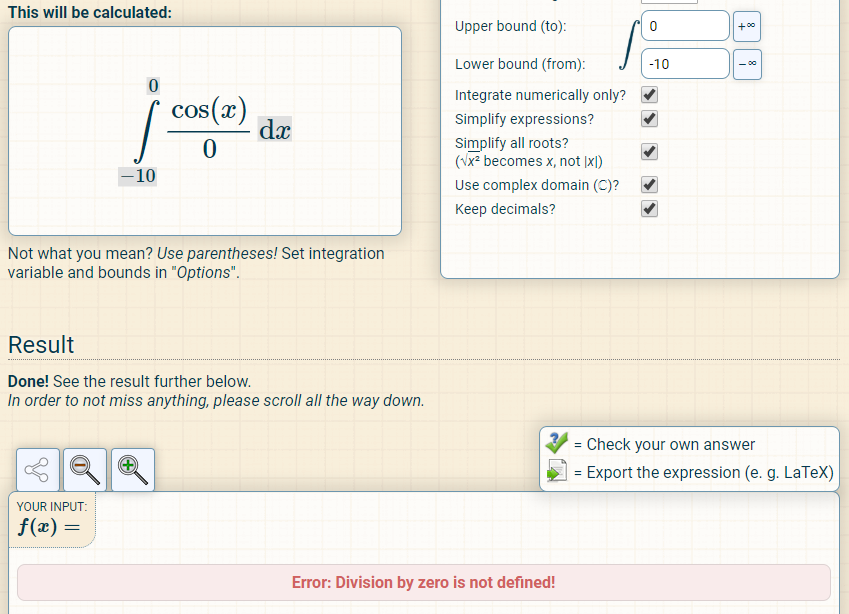
\includegraphics[scale=0.7]{images/Case3}
	\captionof{figure}{Test Case 3}
	\vspace{1cm}
\end{center}


\begin{center}
	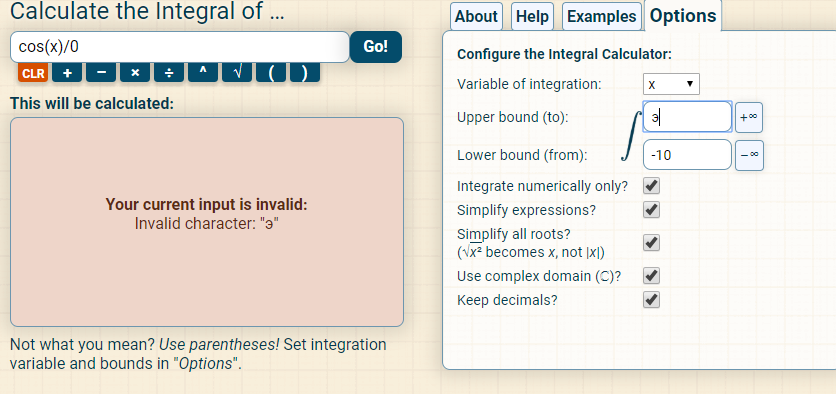
\includegraphics[scale=0.7]{images/Case4}
	\captionof{figure}{Test Case 4}
	\vspace{1cm}
\end{center}

\subsection{Task 4 - Emphasis on tests which get errors}

The tests that can get errors in the tested system are :

\begin{itemize}
	\item Non-valid mathematical expressions;
	\item Semantically non-valid expressions;
	\item Not supported character sets;
	\item Options which are beyond the domain of the used functions;
\end{itemize}

\clearpage